\documentclass[10pt]{beamer}
\usetheme[
%%% options passed to the outer theme
%    hidetitle,           % hide the (short) title in the sidebar
%    hideauthor,          % hide the (short) author in the sidebar
%    hideinstitute,       % hide the (short) institute in the bottom of the sidebar
%    shownavsym,          % show the navigation symbols
%    width=2cm,           % width of the sidebar (default is 2 cm)
%    hideothersubsections,% hide all subsections but the subsections in the current section
%    hideallsubsections,  % hide all subsections
    left               % right of left position of sidebar (default is right)
%%% options passed to the color theme
%    lightheaderbg,       % use a light header background
  ]{AAUsidebar}

% If you want to change the colors of the various elements in the theme, edit and uncomment the following lines
% Change the bar and sidebar colors:
%\setbeamercolor{AAUsidebar}{fg=red!20,bg=red}
%\setbeamercolor{sidebar}{bg=red!20}
% Change the color of the structural elements:
%\setbeamercolor{structure}{fg=red}
% Change the frame title text color:
%\setbeamercolor{frametitle}{fg=blue}
% Change the normal text color background:
%\setbeamercolor{normal text}{bg=gray!10}
% ... and you can of course change a lot more - see the beamer user manual.


\usepackage[utf8]{inputenc}
\usepackage[english]{babel}
\usepackage[T1]{fontenc}
\usepackage{multimedia}
\usepackage{graphicx} % enable fitting figures
\usepackage{wrapfig}
\usepackage{adjustbox}
% Or whatever. Note that the encoding and the font should match. If T1
% does not look nice, try deleting the line with the fontenc.
\usepackage{helvet}
\usepackage{tikz}
\usetikzlibrary{shapes,shapes.geometric, arrows,positioning,calc}
\tikzset{
	block/.style = {draw, fill=white, rectangle, minimum height=3em, minimum width=3em},
	tmp/.style  = {coordinate}, 
	sum/.style= {draw, fill=white, circle, node distance=1cm},
	input/.style = {coordinate},
	output/.style= {coordinate},
	pinstyle/.style = {pin edge={to-,thin,black}
	}
}

\usepackage{amsmath}
\usepackage{amssymb}

% colored hyperlinks
\newcommand{\chref}[2]{%
  \href{#1}{{\usebeamercolor[bg]{AAUsidebar}#2}}%
}

\title[Modelling and Networked Control of Water Distribution Networks]% optional, use only with long paper titles
{This is the title i think}

% \subtitle{}  % could also be a conference name

\date{\today}

\author[CA834] % optional, use only with lots of authors
{
  CA834
}
% - Give the names in the same order as they appear in the paper.
% - Use the \inst{?} command only if the authors have different
%   affiliation. See the beamer manual for an example

\institute[
%  {\includegraphics[scale=0.2]{aau_segl}}\\ %insert a company, department or university logo
  Control and Automation\\
  Aalborg University\\
  Denmark
] % optional - is placed in the bottom of the sidebar on every slide
{% is placed on the title page
  Control and Automation, Group 834\\
  Aalborg University\\
  Denmark
  
  %there must be an empty line above this line - otherwise some unwanted space is added between the university and the country (I do not know why;( )
}


% specify a logo on the titlepage (you can specify additional logos an include them in 
% institute command below
\pgfdeclareimage[height=1.5cm]{titlepagelogo}{AAUgraphics/aau_logo_new} % placed on the title page
%\pgfdeclareimage[height=1.5cm]{titlepagelogo2}{graphics/aau_logo_new} % placed on the title page
\titlegraphic{% is placed on the bottom of the title page
  \pgfuseimage{titlepagelogo}
%  \hspace{1cm}\pgfuseimage{titlepagelogo2}
}


\begin{document}
% the titlepage
{\aauwavesbg%
\begin{frame}[plain,noframenumbering] % the plain option removes the sidebar and header from the title page
  \titlepage
\end{frame}}


%%%%%%%%%%%%%%%%

% TOC
\begin{frame}{Agenda}{}
\tableofcontents
\end{frame}






% ======================================================================
% Inputs for topics here!

\section{Introduction}
\begin{frame}{Introduction}{What is a Reefer Trailer}
 		\begin{columns}
 		\begin{column}{.5\textwidth}
 			\textbf{Reefer trailer}
	 			\begin{itemize}
		 			\item Transport of perishable goods
		 			\item On land, via trucks
		 			\item Self supplying, batteries			
		 		\end{itemize} \bigskip\bigskip
 			\textbf{Role} 
		 		\begin{itemize}
		 			\item Critical link in global logistics
		 			\item Extends durability of cargo
		 			\item To and from distribution centers			
		 		\end{itemize}
 		\end{column}
 		\begin{column}{.5\textwidth}
 				\raggedleft
 				\includegraphics[width=.95\textwidth]{../Graphics/3d_draw_trailer.pdf}
				\centering
				\includegraphics[width=0.45\textwidth]{../Graphics/Transportation_networks.pdf}
 		\end{column}
 	\end{columns}	
\end{frame}

%%%%%%%%%%%%%%%%

\begin{frame}{Introduction}{Efficiency Motivation}
	\begin{itemize}
		\item Increased energy efficiency $\rightarrow$ less power required $\rightarrow$ reduced operational costs  
		\item Smaller batteries $\rightarrow$ reduced capital costs		
	\end{itemize}\bigskip
	\textbf{Efficiency of Reefer Trailers: UN's Sustainable Development Goals}
	\begin{itemize}	
		\item 2nd: Food supply
		\begin{itemize}
			\item Cost of fresh food is correlated with transport costs
			\item Reduced costs increase access to fresh foods for low income people		
		\end{itemize}
		\item 7th: Energy efficiency
		\begin{itemize}
			\item Decreased CO2 emissions per transported good
			\item Decreased use of rare metals for batteries	
		\end{itemize}
	\end{itemize}	
\end{frame}

%%%%%%%%%%%%%%%%%
\begin{frame}{Introduction}{Concept of Reefer trailer}
%	\textbf{Some text}
	\begin{itemize}
		\item Insulated trailer
		\item Heat need be removed from cargo through airflow	
	\end{itemize}
	\includegraphics[width=1\textwidth]{../Graphics/Trailer_airflow.pdf}
	\begin{itemize}
		\item High-Fidelity (Hi-Fi) simulation model of trailer is supplied by BITZER
		\item Hi-Fi model is implemented with PID controllers
	\end{itemize}
\end{frame}

%%%%%%%%%%%%%%%%%
\begin{frame}{Introduction}{Problem Definition}
	\textbf{Problem Definition:} Can a MIMO controller be designed to improve energy efficiency of the reefer trailer Hi-Fi simulation model?
	\begin{itemize}
		\item Boiled down a bit. 
		\item Stable MIMO controller
	\end{itemize}
\end{frame}

%%%%%%%%%%%%%%%%%
\begin{frame}{System Description}{Refrigeration circuit}
	\textbf{Two stage refrigeration system with flash tank}
	\begin{itemize}
		\item Increased efficiency compared to one stage system 
		\item Subcooling throttle is not modeled
		\item Controlled inputs and outputs
		\begin{itemize}
			\item 5 inputs, 2 outputs
		\end{itemize}
		\item Load delivers heat to evaporator
	\end{itemize}
\begin{figure}[h]
	\centering
	\begin{minipage}{0.6\textwidth}
		\centering
		\includegraphics[width=1\textwidth]{../Graphics/HVAC_Diagram_Fans.pdf} % first figure itself
%		\caption{Illustration of two stage refrigeration circuit}
%		\label{fig:HVAC_Diagram}
	\end{minipage}\hfill
	\begin{minipage}{0.4\textwidth}
		\centering
		\includegraphics[width=1.05\textwidth]{../Graphics/Flash_Tank_P-h_Diagram} % second figure itself
%		\caption{Illustration of p-h diagram of two stage refrigeration circuit}
%		\label{fig:p-h_diagram}
	\end{minipage}
\end{figure}
\end{frame}

%%%%%%%%%%%%%%%%%
%\begin{frame}{System description}{Entire System}
%	
%	\textbf{Some text}
%	\begin{itemize}
%		\item Item
%	\end{itemize}
%\end{frame}

%%%%%%%%%%%%%%%%%%
%\begin{frame}{System description}{}
%	\textbf{Some text}
%	\begin{itemize}
%		\item Item
%	\end{itemize}
%\end{frame}
%
%%%%%%%%%%%%%%%%%%
%\begin{frame}{System description}{}
%	\textbf{Some text}
%	\begin{itemize}
%		\item Item
%	\end{itemize}
%\end{frame}

%%%%%%%%%%%%%%%%%%
%\begin{frame}{Next slide title}{Next slide subtitle}
%	\textbf{Some text}
%	\begin{itemize}
%		\item Item
%	\end{itemize}
%\end{frame}
%
%%%%%%%%%%%%%%%%%%
%\begin{frame}{Next slide title}{Next slide subtitle}
%	\textbf{Some text}
%	\begin{itemize}
%		\item Item
%	\end{itemize}
%\end{frame}
%
%%%%%%%%%%%%%%%%%%
%\begin{frame}{Next slide title}{Next slide subtitle}
%	\textbf{Some text}
%	\begin{itemize}
%		\item Item
%	\end{itemize}
%\end{frame}
%
%%%%%%%%%%%%%%%%%%

\section{Modeling}
\begin{frame}{Modelling}{Introduction}
	A model of the refrigeration system is derived, linearised and further developed for observer based control.
	\begin{itemize}
		\item \textbf{Main goal:} Capture dynamics important for the box air temperature (main control objective)
		\begin{itemize}
			\item Thermal masses: Trailer box, cargo, evaporator, condenser.
		\end{itemize}
		\item \textbf{Modular approach:} Inputs, outputs, internal equations/states
		\item \textbf{Slow vs. fast dynamics:} States or algebraic equations
		\begin{itemize}
			\item Including faster dynamics yield more accurate model yet it is unnecessary from control perspective.
		\end{itemize}		
	\end{itemize}
\end{frame}



%%%%%%%%%%%%%%%%%

\begin{frame}{Modelling}{Component Models}
	Each component is modelled separately. The components are:
	\begin{itemize}
		\item Expansion Valve
		\item Pipe joining junction
		\item Compressor
		\item Condenser
		\item Flash tank
		\item Evaporator
		\item Box
	\end{itemize}
\end{frame}



%%%%%%%%%%%%%%%%%

\begin{frame}{Modelling}{Expansion Valve}
	\textbf{Purpose:} Lower pressure of liquid refrigerant from flash tank to evaporator.
	\begin{itemize}
		\item Adiabatic process: Modelled algebraicly
	\end{itemize}
	Flow through valve:
	\begin{equation} \label{eq:ExpansionValve_Alt}
		\begin{split}
			\dot{m} & = f_p(\Theta) K  \sqrt{\frac{1}{v_{in}} (p_{in} - p_{out})} \\
		\end{split}
	\end{equation}

	Table lookup:
	\begin{equation} \label{eq:ExpansionValve_vin}
		v_{in} = \mathcal{Z}(h_{in}, p_{in})
	\end{equation}
\end{frame}



%%%%%%%%%%%%%%%%%

\begin{frame}{Modelling}{Pipe joining junction}
	\textbf{Purpose:} Join refrigerant flows from between compressor stage 1 and two and the flash tank.
	\begin{itemize}
		\item States: $M$
	\end{itemize}
	Mass balance:
	\begin{equation}
	 \frac{dM}{dt} = \dot{m}_{in1} + \dot{m}_{in2} - \dot{m}_{out}       \label{eq:PipeJoiningJunction_ChangeOfMass}
	\end{equation}
	Enthalpy out:
	\begin{equation} \label{eq:PipeJoiningJunction_Enthalpy}
		h_{out} = \frac{h_{in1} \cdot \dot{m}_{in1} + h_{in2} \cdot \dot{m}_{in2}}{ \dot{m}_{in1} + \dot{m}_{in2} }
	\end{equation}
	
\end{frame}



%%%%%%%%%%%%%%%%%

\begin{frame}{Modelling}{Compressor}
	\textbf{Purpose:} Generate pressure sufficient for refrigerant flow and condenser heat flow
	\begin{itemize}
		\item Two compressor stages
		\item Only difference: Stage 2 has half the internal volume of stage 1
		\item Modelled as reciprocating (piston) compressor
		\item Modelled algebraicly - Fast dynamics do not affect slow evaporator dynamics 
	\end{itemize}
	Flow through compressor and enthalpy out
	\begin{align}
		\dot{m} &= \left(\frac{V_1}{v_1} - \frac{V_C}{v_2}\right) \frac{\omega}{2} \label{eq:comp_mass_flow} \\
		h_{out} &= \Upsilon(T_{out}, p_{out}) \label{eq:comp_enthalpy}
	\end{align}
\end{frame}

%%%%%%%%%%%%%%%%%

\begin{frame}{Modelling}{Condenser}
	\textbf{Purpose:} Exchange heat from hot vapour refrigerant to outside ambient air 
	\begin{itemize}
		\item Modelled as one Control Volume (CV)
		\item States: $M_r$ and $T_m$
	\end{itemize}
	\begin{figure}[h!]
		\centering
		\includegraphics[width=1\textwidth]{../Graphics/Condenser.pdf}
		\caption{Diagram of condenser control volume}
		\label{fig:condenser_CV}
	\end{figure}
\end{frame}

\begin{frame}{Condenser}{Equations}
	Energy balance:
	\begin{equation}
		h_{out} = h_{in} - \frac{Q_{rm}}{\dot{m}_{in}} \label{eq:Condenser_Enthalpy}
	\end{equation}
	Refrigerant mass balance:
	\begin{equation}
		\frac{dM_r}{dt} 	 = \dot{m}_{in}(t) - \dot{m}_{out}(t) \label{eq:Condenser_ChangeOfMass}
	\end{equation}
	Metal temperature:
	\begin{equation}
		\frac{dT_m}{dt} 	 = \frac{Q_{rm} - Q_{ma}}{M_m \cdot Cp_m} \label{eq:Condenser_ChangeOfTemperature}
	\end{equation}
\end{frame}




%%%%%%%%%%%%%%%%%

\begin{frame}{Modelling}{Flash tank}
	\textbf{Purpose:} Separate vapour and liquid refrigerant after condenser throttle valve (CDV)
	\begin{itemize}
		\item Modelled algebraicly
		\item Pressures out = in
	\end{itemize}
	\begin{figure}[h!]
		\centering
		\includegraphics[width=0.7\textwidth]{../Graphics/Flash_tank.pdf}
%		\caption{Diagram of Flash tank control volumes}
		\label{fig:flash_tank_CV}
	\end{figure}
	Mass balance:
\begin{equation}
	\dot{m}_{v} = \dot{m}_{lv} - \dot{m}_{l}  \label{eq:Flash_tank_massflow}
\end{equation}
Enthalpies:
\begin{equation}
	h_{l} = \mathcal{M}(p) \hspace{0.8cm} h_{v} = \mathcal{N}(p)
\end{equation}
\end{frame}



%%%%%%%%%%%%%%%%%

\begin{frame}{Modelling}{Evaporator}
	\textbf{Purpose:} Exchange heat from box air to cold liquid refrigerant
	\begin{itemize}
		\item Superheat is important control objective
		\item Modelled with two CVs: liquid-vapour and vapour
		\item Pressure out is simplified to being pressure in
		\item States: $T_{mlv}$, $T_{mv}$, $M_{lv}$, $M_{v}$ and $T_{v}$
	\end{itemize}
	
	\vspace{0.4cm}
	\begin{figure}[h!]
		\centering
		\includegraphics[width=1\textwidth]{../Graphics/Evaporator_CV_diagram.pdf}
		\caption{Diagram of evaporator liquid-vapour and liquid CVs split by $\sigma$}
		\label{fig:evap_CV}
	\end{figure}

\end{frame}

\begin{frame}{Evaporator}{Equations}
	Moving boundary and specific volume out
	\begin{equation}
		\sigma = \frac{M_{lv} \cdot v_1}{V_i} \label{eq:Evaporator_boundary}
	\end{equation}
	Liquid-vapour temperature:
	\begin{equation}
		\frac{dT_{mlv}}{dt}  = \frac{Q_{amlv}-Q_{mlv} + Q_{mvmlv}}{M_m \cdot \sigma \cdot Cp_m} \label{eq:evap_dT_ml}
	\end{equation}
	Vapour metal temperature:
	\begin{equation}
		\frac{dT_{mv}}{dt} = \frac{Q_{amv} - Q_{mv} - Q_{mvmlv}}{M_m \cdot (1 - \sigma) \cdot Cp_m} \label{eq:evap_dT_mv}
	\end{equation}
	Mass balances:
	\begin{equation} \label{eq:evap_dMlv}
		\frac{dM_{lv}}{dt} = \dot{m}_{in} - \dot{m}_{dew} \hspace{0.8cm}  \frac{dM_v}{dt} = \dot{m}_{dew} - \dot{m}_{out}
	\end{equation}
	Vapour refrigerant temperature:
	\begin{equation}\label{eq:tv_initial}
		\frac{dT_{v}}{dt} = \bar{T_v} - T_v
	\end{equation}

\end{frame}

%%%%%%%%%%%%%%%%%

\begin{frame}{Modelling}{Box}
	\textbf{Purpose:} Allow for convective heat transfer between cargo and circulating air
	\begin{itemize}
		\item Contains greatest thermal masses
		\item States: $T_{air}$, $T_{box}$ and $T_{cargo}$
	\end{itemize}
	\begin{figure}[h!]
		\centering
		\includegraphics[width=0.8\textwidth]{../Graphics/Box.pdf}
		\caption{Simplified diagram of trailer box}
		\label{fig:box_diagram}
	\end{figure}


\end{frame}

\begin{frame}{Box}{Equations}
	Air, box and cargo temperatures:
	\begin{align}
		\frac{dT_{air}}{dt} &= \frac{Q_{ca} + Q_{ba} + Q_{fan} -Q_{cool}}{M_{air} \cdot Cp_{air}} \label{eq:box_dT_air} \\
		\frac{dT_{box}}{dt} &= \frac{Q_{amb} - Q_{ba}}{M_{box} \cdot Cp_{box}} \label{eq:box_dT_box} \\
		\frac{dT_{cargo}}{dt} &= \frac{-Q_{ca}}{M_{cargo} \cdot Cp_{cargo}} \label{eq:box_dT_cargo}
	\end{align}
	Heat flows:
	\begin{align}
		Q_{cool}   & = Cp_{air} \cdot \dot{m}_{air} \cdot (T_{ret} - T_{sup})	\label{eq:box_Qcool} \\
		Q_{amb}    & = (T_{ambi} - T_{box}) \cdot U A_{amb}						\label{eq:box_Qab}   \\
		Q_{ba}     & = (T_{box} - T_{air}) \cdot U A_{ba}						\label{eq:box_Qba}   \\
		Q_{ca}     & = (T_{cargo} - T_{air}) \cdot U A_{ca}                  	\label{eq:box_Qca}
	\end{align}
\end{frame}

%%%%%%%%%%%%%%%%%

\begin{frame}{Modelling}{Formulating non-linear state-space model}
	A non-linear state space model is formulated
	\begin{itemize}
		\item All state equations equations are collected in a $f(x,u)$ vector
		\item Algebraic equations are constraints
	\end{itemize}
	State vector and input vector:
	\begin{equation}  \label{eq:xu}
		\begin{split}
			x & = [M_{pjj}	\;
				M_{con} \;
				T_m \;
				\dot{m}_{air}\;
				T_{mlv}      \;
				T_{mv}       \;
				M_{lv}       \;
				M_v          \;
				T_{air}      \;
				T_{box}      \;
				T_{cargo}    \;
				T_v]^T \\
			u & = [\omega	\;
				\Theta_1	\;
				\Theta_2     \;
				U_{fan_1}    \;
				U_{fan_2}]^T \\
		\end{split}
	\end{equation}

\end{frame}



%%%%%%%%%%%%%%%%%

\begin{frame}{Modelling}{Non-linear state-space system}
	\begin{figure}[h!]
		\centering
		\includegraphics[width=1\textwidth]{Graphics/f_x_u.jpeg}
		\label{fig:f_x_u}
	\end{figure}
\end{frame}





%%%%%%%%%%%%%%%%%

\begin{frame}{Modelling}{Component Input/Output relationship}
	\begin{itemize}
		\item Red: Missing, Blue: Unused.
		\item Pressure/flow input/output setup leads to problems
		\item Current model setup leads to problems e.g. condenser throttle valve
	\end{itemize}
	\begin{figure}[h!]
		\centering
		\includegraphics[width=1\textwidth]{../Graphics/Block_Diagram_inout_flowValveVersion.pdf}
		\label{fig:Block_diagram_inout}
	\end{figure}
	
\end{frame}




%%%%%%%%%%%%%%%%%

\begin{frame}{Modelling}{}
	
\end{frame}



%%%%%%%%%%%%%%%%%

\begin{frame}{Modelling}{}
	
\end{frame}



%%%%%%%%%%%%%%%%%

\begin{frame}{Modelling}{}
	
\end{frame}



%%%%%%%%%%%%%%%%%

\begin{frame}{Modelling}{}
	
\end{frame}



%%%%%%%%%%%%%%%%%

\begin{frame}{Modelling}{}
	
\end{frame}



%%%%%%%%%%%%%%%%%

\begin{frame}{Modelling}{}
	
\end{frame}







\section{Controller}
\begin{frame}{Controller design}{Optimal control}
	 \textbf{Definition of optimality}
	 \begin{itemize}
	 	\item Cost function
	 	\item Weighting of variables
	 	\item Horizons
	 	\item Constraints
	 	\item Benefits in comparison to pole-placement 
	 \end{itemize}
 
\begin{equation} \label{eq:lqr_cost_fcn}
	J = \int_0^{\infty} \left(x^TQx + u^TRu + 2x^TNu\right)dt
\end{equation}

\end{frame}

%%%%%%%%%%%%%%%%%%%%%%%%%%%%%%%%%%%%%%%%%%%%%%%%%%%

\begin{frame}{Controller design}{Linear Quadratic Regulator}
	 \textbf{Linear Quadratic Regulator}
	\begin{itemize}
		\item Cost function
		\item Infinite-horizon 
		\item Feedback law
		\item Drawbacks
	\end{itemize}

\begin{equation} \label{eq:lqr_cost_fcn}
	J = \int_0^{\infty} \left(x^TQx + u^TRu\right)dt
\end{equation}
\begin{equation} \label{eq:lqr_cost_fcn}
	u = -Kx
\end{equation}

\begin{equation} \label{eq:lqr_K}
	K = -R^{-1}B^{T}P
\end{equation}

where P is the unique solution to the algebraic Ricatti equation
\begin{equation} \label{eq:ricatti}
	A^TP + PA - PBR^{-1}B^TP+Q = 0
\end{equation}

\end{frame}


%%%%%%%%%%%%%%%%%%%%%%%%%%%%%%%%%%%%%%%%%%%%%%%%%%%

\begin{frame}{Controller design}{Linear Quadratic Regulator}
\begin{equation}
	Q =
	\left(\begin{array}{cccccccc}
		1 & 0 & 0 & 0 & 0 & 0 & 0 & 0  \\
		0 & 1 & 0 & 0 & 0 & 0 & 0 & 0  \\
		0 & 0 & 1 & 0 & 0 & 0 & 0 & 0  \\
		0 & 0 & 0 & 1 & 0 & 0 & 0 & 0  \\
		0 & 0 & 0 & 0 & 2 & 0 & 0 & 0  \\
		0 & 0 & 0 & 0 & 0 & 1 & 0 & 0  \\
		0 & 0 & 0 & 0 & 0 & 0 & 2 & 0  \\
		0 & 0 & 0 & 0 & 0 & 0 & 0 & 1
	\end{array}\right)
	\text{  and  }
	R =
	\left(\begin{array}{cc}
		1 & 0  \\
		0 & 0.025
	\end{array}\right)
\end{equation}

\medskip

\begin{equation}
	K =
	\left(\begin{array}{cccccccccc}
		-0.0784 &  -0.0140 &  -0.0203 &   1.1457 &  -0.1743 &  -0.1021 &  -0.6274 &   0.0049 \\
		0.5679 &   0.0786 &   0.1447 &  -4.0389 &   0.7489 &   0.4246 &   2.5119 &   0.0041
	\end{array}\right)
\end{equation}
	
\end{frame}

%%%%%%%%%%%%%%%%%%%%%%%%%%%%%%%%%%%%%%%%%%%%%%%%%%%%%%%%%%%%%%%%%%%%

\begin{frame}{Controller design}{Observer design}
	\textbf{Observer structure}
	\begin{itemize}
		\item Luenberger observer
		\item Separation Principle
		\item Observer pole placement
	\end{itemize}


\begin{equation} \label{eq:obs_error_dot}
	\dot{e} = (A - LC)e
\end{equation}
\begin{figure}[h!]
	\centering
	\includegraphics[width=0.5\textwidth]{../Graphics/Observer_diagram.pdf}
	\caption{Observer structure}
	\label{fig:obs_struct}
\end{figure}
\end{frame}




%%%%%%%%%%%%%%%%%

\section{Robustness Analysis}
\begin{frame}{Robustness Analysis}{Uncertainty}
	 \textbf{A parameter that will likely vary is the heat transfer coefficient of the cargo }$UA_{ca}$
	 \begin{itemize}
	 	\item Packaging differ
	 	\item Cargo differ
	 \end{itemize} \bigskip
 	\textbf{Stability with a linearly varying parameter can be investigated using LMI's for parameter space}
 	\begin{itemize}
 		\item Checking stability for corner cases guarantee stability in parameter space $\rightarrow$ robust stability! 
 		\item Uncertainty assumed to be $\pm 20 \%$
		\begin{itemize}
			\item Perturbed system was shown to be stable for corner cases
		\end{itemize}
 	\end{itemize}
\end{frame}

%%%%%%%%%%%%%%%%%

\begin{frame}{Robustness Analysis}{Stability}
	For a linear system
	\begin{equation*} \label{eq:lqr_sys}
		\begin{split}
			\dot{x} 	& = Ax + Bu \\
			y 	& = Cx
		\end{split}
	\end{equation*}
	The system is stable iff a P exists that satisfies 
	\begin{equation*} \label{eq:rob_lyapunov_stability}
		\begin{split}
			A^TP+PA &< 0 \\
			P &> 0
		\end{split}
	\end{equation*}
	
	And if a system with uncertainty is stable for all pertubations, it is robust stable. 
	Corner cases for perturbed system:
	\begin{flalign*}
		\hspace{1cm} \bar{A}_{\Delta max} \! ^T \: P + P \:\bar{A}_{\Delta max} &< 0 \text{, $\;$ (+20\% perturbation on $U A_{ca}$)} &\\
		\hspace{1cm} \bar{A}_{\Delta min} \! ^T \: P + P \:\bar{A}_{\Delta min} &< 0 \text{, $\;$ (-20\% perturbation on $U A_{ca}$)} &\\
		P &> 0
	\end{flalign*} 
\end{frame}

%%%%%%%%%%%%%%%%%

\begin{frame}{Uncertainty representation}
	With the system represented as,
		\begin{equation*}
			G = \left\lbrack \begin{array}{cc}
				A_{nom} & B\\
				C & D
			\end{array}\right\rbrack
		\end{equation*}
	The perturbed system can be represented as
		\begin{equation*}
			G_p = G + W\Delta, \quad |\Delta|\leq 1
		\end{equation*}
	where
		\begin{equation*} 
			A_{nom} =
			\begin{bmatrix}
				a_{11} & \cdots &  a_{1n} & \\
				\vdots & \ddots & \vdots & \\
				a_{n1} & \cdots & a_{nn} &
			\end{bmatrix}, W = \left\lbrack \begin{array}{cc}
			W_A & 0\\
			0 & 0 \end{array}\right\rbrack 
		\end{equation*}
	and
\end{frame}

%%%%%%%%%%%%%%%%%



\begin{frame}{Uncertainty Representation}{}
	\begin{equation*}
		W_A = 0.2\begin{bmatrix}
			0      & \cdots & \cdots & \cdots     & \cdots     & 0      \\
			\vdots & \ddots & \cdots & UA_{ca}k_1 & UA_{ca}k_3 & \vdots \\
			\vdots & \vdots & \ddots & UA_{ca}k_2 & UA_{ca}k_4 & \vdots \\
			\vdots & \vdots & \vdots & \ddots     & \cdots     & \vdots \\
			\vdots & \vdots & \vdots & \vdots     & \ddots     & \vdots \\
			0      & \cdots & \cdots & \cdots     & \cdots     & 0
		\end{bmatrix}
	\end{equation*}
	\begin{figure}[h!]
		\centering
		\resizebox{\columnwidth}{!}{
				\begin{adjustbox}{max totalsize={.9\textwidth}{.7\textheight},center}
	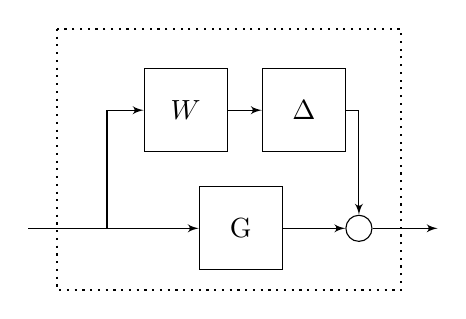
\begin{tikzpicture}[node distance=2.5cm,>=latex']
	% ========================== Nodes ============================
	% Nodes in upper vertical line
	\node [input, name=rinput] (rinput) {};
	\node [tmp, right of=rinput, node distance = 1cm] (tmpadd1){};
	\node [tmp, above of=tmpadd1, node distance = 1.5cm] (tmpadd2){};
	\node [block, right of=tmpadd2, node distance = 1cm] (omegaA) {$W$};
	\node [block, right of=omegaA, node distance = 1.5cm] (deltaA) {$\Delta$};
%	\node [sum, right of=tmpadd1] (sum1) {};
	\node [block, right of=tmpadd1, node distance = 1.7cm] (G) {G};
	\node [sum, right of=G, node distance =1.5cm] (sum2) {};
	\node [tmp, above of=sum2, node distance = 1.5cm] (tmpadd3){};
	\node [tmp, right of=sum2, node distance = 1cm] (tmpadd4){TEST};
	
	
%	\node [tmp, right of=tmpadd4, node distance = 1.5cm] (tmpmul1){};
%	\node [tmp, above of=tmpmul1, node distance = 2.5cm] (tmpmul2){};
%	\node [block, right of=tmpmul2, node distance = 1cm] (omegaI) {$\omega_I$};
%	\node [block, right of=omegaI, node distance = 1.5cm] (deltaI) {$\Delta_I$};
%	%	\node [sum, right of=tmpmul1] (sum1) {};
%
%	\node [sum, right of=tmpmul1, node distance =4cm] (sum3) {};
%	\node [tmp, above of=sum3, node distance = 2.5cm] (tmpmul3){};
%	\node [tmp, right of=sum3, node distance = 1cm] (tmpmul4){TEST};
%	\node [block, right of=sum3, node distance = 2cm] (G2) {G2};
%	
	\draw[thick, dotted] ($(G.north west)+(-1.8, 2)$) rectangle  ($(G.south east)+(1.5, -0.25)$);
%	\node[above of =tmp0, node distance =1.1cm](sys_txt) {System};
%	
	% ========================== Lines ============================

	\draw [-] (rinput) -- (tmpadd1);
	\draw [->] (tmpadd1) -- (G);
	\draw [->] (G) -- (sum2);
	\draw [->] (sum2) -- (tmpadd4);

	
	% Lines for additive uncertainty
	\draw [-] (tmpadd1) -- (tmpadd2);
	\draw [->] (tmpadd2) -- (omegaA);
	\draw [->] (omegaA) -- (deltaA);
	\draw [-] (deltaA) -- (tmpadd3);
	\draw [->] (tmpadd3) -- (sum2);
	
%	% Lines for multiplicative uncertainty
%	\draw [-] (tmpmul1) -- (tmpmul2);
%	\draw [->] (tmpmul2) -- (omegaI);
%	\draw [->] (omegaI) -- (deltaI);
%	\draw [-] (deltaI) -- (tmpmul3);
%	\draw [->] (tmpmul3) -- (sum3);

%	
%	
\end{tikzpicture}
\end{adjustbox}}
		\label{fig:tikzControlStrat}
	\end{figure}
\end{frame}


\section{Test - Controller with Linear Model}
\begin{frame}{Test results}{Linear model test}	 
	 \textbf{Test of reduced linear model for control of full linear model}
	 \begin{itemize}
	 	\item Kalman decomposition and LQR controller verification
	 \end{itemize}
 

 \begin{figure}[h!]
 	\centering
 	\includegraphics[width=1\textwidth]{../Graphics/fig_stateInput10h.png}

 	\label{fig:sim_stateInput10h}
 \end{figure}
 
\end{frame}


%%%%%%%%%%%%%%%%%%%%%%%%%%%%%%%%%%

%\begin{frame}{Next slide title}{Next slide subtitle}
%	 \textbf{Some text}
%	\begin{itemize}
%		\item Item
%	\end{itemize}
%\end{frame}

%%%%%%%%%%%%%%%%%

\section{Test - Controller with Hi-Fi Model}
\begin{frame}{Test results}{HiFi model control}
	 \textbf{Test setup}
	 \begin{figure}[h!]
	 	\centering
	 	\includegraphics[width=0.8\textwidth]{../Graphics/HiFi_simulation_test_diagram.pdf}
	 	\label{fig:test_setup}
	 \end{figure}
 \begin{itemize}
 	\item No disturbance
 	\item Sine disturbance
 	\item Step disturbance
 \end{itemize}
\end{frame}

%%%%%%%%%%%%%%%%%

\begin{frame}{Test results}{HiFi model control}
	\textbf{No disturbance - controlled outputs}
	\begin{figure}[H]
		\centering
		\includegraphics[width=0.8\textwidth]{../Graphics/fig_LQRvsKresten_noDist.png}
	\end{figure} 
\end{frame}

%%%%%%%%%%%%%%%%%

\begin{frame}{Test results}{HiFi model control}
	 \textbf{No disturbance - control signals}
	\begin{figure}[H]
		\centering
		\includegraphics[width=0.8\textwidth]{../Graphics/fig_inputs_noDist.png}
	\end{figure}
\end{frame}

%%%%%%%%%%%%%%%%%

\begin{frame}{Test results}{HiFi model control}
	\textbf{Sine disturbance - controlled outputs}
	\begin{figure}[H]
		\centering
		\includegraphics[width=0.8\textwidth]{../Graphics/fig_LQRvsKresten_sineDist.png}
	\end{figure} 
\end{frame}

%%%%%%%%%%%%%%%%%

\begin{frame}{Test results}{HiFi model control}
	\textbf{Sine disturbance - control signals}
	\begin{figure}[H]
		\centering
		\includegraphics[width=0.8\textwidth]{../Graphics/fig_inputs_sineDist.png}
	\end{figure}
\end{frame}

%%%%%%%%%%%%%%%%%

\begin{frame}{Test results}{HiFi model control}
	\textbf{Step disturbance - controlled outputs}
	\begin{figure}[H]
		\centering
		\includegraphics[width=0.8\textwidth]{../Graphics/fig_LQRvsKresten_stepDist.png}
	\end{figure} 
\end{frame}

%%%%%%%%%%%%%%%%%

\begin{frame}{Test results}{HiFi model control}
	\textbf{Step disturbance - control signals}
	\begin{figure}[H]
		\centering
		\includegraphics[width=0.8\textwidth]{../Graphics/fig_inputs_stepDist.png}
	\end{figure}
\end{frame}

%%%%%%%%%%%%%%%%%





\section{Conclusion}
\begin{frame}{Conclusion}
%	 \textbf{Some text}
	 \begin{itemize}
	 	\item First principle linear state space model 
	 	\item Greatly reduced model size compared to previous work
	 	\item Low amount of measurements used
	 	\item Stable oberserver based LQR controller 
	 	\item Poor disturbance rejection
	 	\item Equivalent energy efficiency
	 \end{itemize}
\end{frame}

%%%%%%%%%%%%%%%%%

\begin{frame}{Next slide title}{Next slide subtitle}
	 \textbf{Some text}
	\begin{itemize}
		\item Item
	\end{itemize}
\end{frame}

%%%%%%%%%%%%%%%%%

\section{Future work and improvements}
\begin{frame}{Future work}
	 \textbf{System model}
	 \begin{itemize}
	 	\item Continued work on component model analysis
	 	\item Improvement of connection between components
	 	\item Inclusion of all controlled variables in the model
	 	\item Increased number of relevant states
	 \end{itemize}
 
 \bigskip
 
 	\textbf{Controller design}
	\begin{itemize}
 		\item Integral action for no steady state error
 		\item MPC design for inclusion of actuator constraints
 		\item Gain scheduling for wider range of control
 	\end{itemize}
\end{frame}










% ======================================================================




\section{References}
\begin{frame}{References}
	\bibliographystyle{ieeetran}
	\bibliography{../../RefLib/CA7Projekt.bib}
\end{frame}

{\aauwavesbg
\begin{frame}[plain,noframenumbering]
  \finalpage{Open for questions!}
\end{frame}}
%%%%%%%%%%%%%%%%

\end{document}
